  %  File:  EGB_algorithm.tex

\documentclass{amsart}
\usepackage{amssymb}
\usepackage{algorithmic}
\usepackage{graphicx}
\usepackage{etoolbox}
\usepackage{setspace}
\usepackage{hyperref}
\usepackage{verbatim}
 
\newtheorem{theorem}{Theorem}[section]
\newtheorem{lemma}[theorem]{Lemma}
\newtheorem{proposition}[theorem]{Proposition}
\newtheorem{corollary}[theorem]{Corollary}
\newtheorem{question}[theorem]{Question}\newtheorem{conjecture}[theorem]{Conjecture}

\theoremstyle{definition}
\newtheorem{definition}[theorem]{Definition}
\newtheorem{example}[theorem]{Example}
\newtheorem{problem}[theorem]{Problem}
\newtheorem{xca}[theorem]{Exercise}
\newtheorem{algorithm}[theorem]{Algorithm}

\theoremstyle{remark}
\newtheorem{remark}[theorem]{Remark}
\newtheorem{criterion}[theorem]{Criterion}

\numberwithin{equation}{section}

\newenvironment{Macaulay2}{ \begin{spacing}{0.4} %\begin{quote}
\smallskip } { \smallskip %\end{quote}
\end{spacing} }

\newcommand{\B}[1]{\mathbb #1}
\newcommand{\C}[1]{\mathcal #1}
\newcommand{\F}[1]{\mathfrak #1}

%    Absolute value notation
\newcommand{\abs}[1]{\lvert#1\rvert}

%    Blank box placeholder for figures (to avoid requiring any
%    particular graphics capabilities for printing this document).
\newcommand{\blankbox}[2]{%
  \parbox{\columnwidth}{\centering
%    Set 
fboxsep to 0 so that the actual size of the box will match the
%    given measurements more closely.
    \setlength{\fboxsep}{0pt}%
    
\fbox{\raisebox{0pt}[#2]{\hspace{#1}}}%
  }%
}

\newcommand{\floor}[1]{\lfloor {#1} \rfloor}
\newcommand{\ceil}[1]{\lceil {#1} \rceil}
\newcommand{\binomial}[2]{\left( 
\begin{array}{c} {#1} \\
                        {#2} \end{array} \right)}
\def\la{\langle}
\def\ra{\rangle}

\newcommand{\lm}{\operatorname{lm}}
\newcommand{\lc}{\operatorname{lc}}
\newcommand{\lt}{\operatorname{lt}}


\newcommand{\rank}{\textit{\rm rank}}
\newcommand{\<}{\langle}
\renewcommand{\>}{\rangle}
\newcommand{\ideal}[1]{\langle #1 \rangle}
\newcommand{\LT}{\operatorname{in}_>}
\newcommand{\Inc}{\operatorname{Inc}(\B N)}
\newcommand{\NF}{\operatorname{NF}}


\begin{document} \title[Algorithms for Equivariant Gr\"obner Bases]
{Algorithms for Equivariant Gr\"obner Bases}

 %   Information for first author 
\author{Christopher J. Hillar}
\address{Redwood Center for Theoretical Neuroscience, University of California, Berkeley}
\email{chillar@msri.org}

\author{Robert Krone}
\address{Georgia Institute of Technology, Atlanta, GA}
\email{krone@math.gatech.edu}

\author{Anton Leykin}
\address{Georgia Institute of Technology, Atlanta, GA}
\email{leykin@math.gatech.edu}

%\thanks{The work of the first author is supported under a National Science Foundation Graduate Research Fellowship.} 

\subjclass{13E05, 13E15, 20B30, 06A07}%

% \keywords{Invariant ideal, well-quasi-ordering, symmetric group, Gr\"obner basis, generating sets}


% \keywords{}

% ----------------------------------------------------------------
\begin{abstract}
 A polynomial ring over a countably infinite number of variables presents some obstacles to computation because it is not Noetherian.  However, often ideals of interest in this setting are endowed with certain symmetry.  If $G$ is an action on the set of variables of the ring, an ideal is $G$-equivariant if it is closed under the action of $G$.  For certain actions, $G$-equivariant ideals are finitely generated up to $G$ action, and moreover there exist equivariant Gr\"obner bases for such ideals. We describe our implementation of an algorithm for computing equivariant Gr\"obner bases in Macaulay2, and include some examples of its application to particular problems.  Additionally we discuss our efforts to improve its run-time, and the obstacles involved.
\end{abstract}

\maketitle

\section{Introduction}
Let $X = \{x_1,x_2,\ldots\}$ be an countably infinite collection of indeterminates.  Fixing a field $k$, let $R = k[X]$ be the polynomial ring with over $k$ with indeterminates $X$.  Let $G$ be a semigroup [*** CHRIS: why not use \textit{monoid} here and throughout?   semigroups don't necessarily have identity elements ***] with a left action on $X$, so there is a natural left action of $G$ on $R$.  For a polynomial $f \in R$ and semigroup element $\sigma \in G$, the action of $g$ on $f$ is defined as
 \[ \sigma\cdot f(x_1,x_2,\ldots) = f(\sigma(x_1),\sigma(x_2),\ldots). \]

Indexing $X$ by the natural numbers, two semigroups of particular interest are
\begin{itemize}
 \item ${\mathfrak S}_{\infty}$, the group of all permutations of $\B N$, and
 \item $\Inc$, the semigroup of all strictly increasing functions $\B N \to \B N$.
\end{itemize}
Other examples of semigroup actions of interest come from indexing the variables in other ways:
\begin{itemize}
 \item Index $X$ by $\B N \times [n]$ for some positive integer $n$ and act with either $\F S_\infty$ or $\Inc$ on only the first index.
 \item Index $X$ by $\B N \times \B N$ and act with either $\F S_\infty$ or $\Inc$ diagonally on both indices.
\end{itemize}


The left actions of $G$ and $R$ on $R$ can be combined into an action of the twisted semigroup ring of $G$ over $R$, denoted $R*G$.  The additive structure of $R*G$ is the same as the semigroup ring $R[G]$.  Multiplication is defined term-wise by 
 \[ f\sigma\cdot g\tau = f\sigma(g)(\sigma\tau) \]
for $f,g\in R$ and $\sigma,\tau\in G$, and extended by linearity.  Note that elements of $R$ and $G$ do not commute with each other in $R*G$, mirroring the lack of commutativity of acting on $R$ by permuting the variables and by multiplying by a polynomial.  $R$ has a natural $R*G$-module structure.

\begin{definition}
 An ideal $I \subseteq R$ is $G$\textit{-equivariant}
(or simply \textit{equivariant}) if \[ GI := \{\sigma f
: \sigma \in G, \ f \in I\} \subseteq I.\]
\end{definition}
$G$-equivariant ideals are exactly the $R*G$-submodules of $R$.

\begin{definition}
$R$ is $G${\em -Noetherian} if it satisfies the ascending chain condition for $G$-equivariant ideals. 
\end{definition}
In particular $G$-Noetherianity implies every $G$-equivariant ideal is finitely generated as an $R*G$-module, which is of particular interest to us.  The notation $\ideal{f_1,\ldots,f_s}_{R*G}$ will be used to denote the equivariant ideal generated by polynomials $f_1,\ldots,f_s$ as an $R*G$-module.

\begin{theorem}\label{onevarfinitegenthm}
$R$ is $\F S_\infty$-Noetherian.  $R$ is $\Inc$-Noetherian.
\end{theorem}

\begin{example}
$I = \<x_1,x_2,\ldots\>_R$ is a $\F S_\infty$-equivariant ideal of $R$.  It can be expressed as $I= \<x_1\>_{R*\F S_\infty}$.
\end{example}

\section{Equivariant Gr\"obner Bases}
In order to define Gr\"obner bases, we give $R$ a monomial order $>$, and impose the following requirement on the relationship between $G$ and the order:
\begin{itemize}
 \item For any monomials $x^\alpha, x^\beta \in R$, and $\sigma \in G$,
\[ x^\alpha > x^\beta \quad \Leftrightarrow \quad \sigma x^\alpha > \sigma x^\beta. \]
\end{itemize}
If this condition is met we say $G$ respects the order $>$.
Note that there is no monomial order which the action of $\F S_\infty$ respects, so we won't be able to define $\F S_\infty$-equivariant Gr\"obner bases.  However there are monomial orders which respect $\Inc$, for example lexicographic order with
\[x_1 < x_2 < x_3 < \cdots.\]
We can use $\Inc$ as a substitute for $\F S_\infty$ using the following fact.
\begin{theorem}
For any finite $F \subset R$, there exists $n$ such that $F \subset k[x_1,\ldots,x_n]$.  Then
 \[ \ideal{F}_{\F S_\infty} = \ideal{\F S_n F}_{\Inc}. \]
\end{theorem}
So any $\F S_\infty$-equivariant ideal generated by $F$ can be represented as a $\Inc$-equivariant ideal with a finite generating set easily constructed from $F$.


\begin{definition}
 A $G$-equivariant Gr\"obner basis for equivariant ideal $I$ with monomial order $>$ that respects $G$ is a set $B \subset I$ such that for any $f \in I$, there is $g \in B$ such that
  \[ \LT f = m\cdot \LT g \]
 for some monomial $m \in R*G$. 
\end{definition}

The normal form of a polynomial $f$ with respect to a set of polynomials $B$, denoted $\NF_B(f)$, is defined in the usual way.  We reduce by an element $g \in B$ if there is some $\sigma \in G$ such that $\sigma \cdot \LT g$ divides $\LT f$.

An implementation issue with this equivariant normal form algorithm is efficiently finding $\sigma \in G$ such that $\sigma \LT g$ divides $\LT f$.  This can be difficult depending on the semigroup action.  In the case of $G = \Inc$ acting on a single index, there is a linear time greedy algorithm, by mapping each variable in $\LT g$ in turn to the first possible variable in $\LT f$ with a large enough exponent.  For $G = \Inc$ acting diagonally on variables indexed by $\B N \times \B N$, we are not aware of a polynomial time algorithm.  Computing $\sigma$ as efficiently as possible is an opportunity for improvement.

\begin{theorem}
Let $B$ be a $G$-equivariant Gr\"obner basis for equivariant ideal $I$.  Then $f \in I$ if and only if $f$ has normal form $0$ with respect to $B$.
\end{theorem}

\section{Equivariant Buchberger algorithm}
If $R$ is $G$-Noetherian, then every equivariant ideal has a finite equivariant Gr\"obner basis.  Without $G$-Noetherianity certain finitely generated ideals may still have a finite equivariant Gr\"obner basis, but this is not guaranteed.  In either case, given a set of generators for an equivariant ideal, we can try to use a variant of the Buchberger algorithm to compute a Gr\"obner basis.

The main departure from the usual Buchberger algorithm comes when computing S-polynomials from a given pair of polynomials $f,h$.  In the standard Buchberger algorithm, there is only one S-polynomial to consider, $S(f,h)$.  In the equivariant case, there is no longer a single S-polynomial which generates all differences $m_1f - m_2h$ where $\LT m_1f = \LT m_2h$ for $m_1,m_2$ monomials in $R*G$.  Instead we need to generate all S-polynomials in the set
 \[ S(Gf,Gh) := \{ S(\sigma f, \tau h): \sigma,\tau \in G\}. \]
Typically this set is infinite, so for the algorithm to succeed we need to impose another requirement on the action of $G$:
\begin{itemize}
 \item For each $f,h \in R$, the set $Gf \times Gh$ is contained in the union of of a finite number of $G$-orbits $G(\sigma_1 f, \tau_1 h),\ldots,G(\sigma_r f, \tau_r h)$, and we can compute the pairs $(\sigma_1,\tau_1),\ldots,(\sigma_r,\tau_r)$.
\end{itemize}

\begin{theorem}
 Fixing $f,h \in R$, there is some $n$ such that $f,h \in k[x_1,\ldots,x_n]$.  Then for any $\sigma', \tau' \in \Inc$, there exist strictly increasing functions $\sigma,\tau: [n] \to [2n]$ and $\rho \in \Inc$ such that
  \[ \rho (\sigma f, \tau h) = (\sigma' f, \tau' h). \]
\end{theorem}

\begin{figure}[h]
  \centering
  \includegraphics[width=.7\textwidth]{incmap.ps}
\end{figure}

Therefore we can consider only S-polynomials of the form $S(\sigma' f,\tau' h)$.  The theorem also holds for $\Inc$ acting on variables indexed by $\B N \times \B N$ or $\B N \times [n]$.  Note that the number of pairs of strictly increasing functions $[n] \to [2n]$ is $\binom{2n}{n}^2$, which is large but finite.

We can make some improvements on the number of S-polynomials considered for each pair $f,h \in B$.  In particular it's not necessary to consider all pairs of increasing maps $[n] \to [2n]$, but just the ways of ``interlacing'' the indices of $f$ and $h$.  These are the pairs $(\sigma,\tau)$ such that $\sigma[n] \cup \tau[n] = [n+r]$ for some $0 \leq r \leq n$.  We call $r$ the number of ``gaps'' in the pair since it is the number of values skipped in the image of each of the two maps.  To count the number of interlacings with $r$ gaps, we can choose any $r$ elements of $[n+r]$ to be $\sigma[n] \setminus \tau[n]$ and any $r$ of the remaining $n$ elements to be $\tau[n] \setminus \sigma[n]$.  So the total number of pairs is
 \[ \sum_{r=0}^{n-1} \binom{n+r}{r}\binom{n}{r}. \]
Note that gap size $n$ can be ruled out.  In this case the variable support of $\sigma f$ and $\tau h$ will be disjoint, and so $S(\sigma f, \tau h)$ will always reduce to zero.

To further reduce the number of S-polynomials considered, we make use of the fact that in practice, most elements of the Gr\"obner basis can be found from examining only the S-polynomials coming from interlacings with gap size 0 or 1.  As a result, at each iteration of the search for new Gr\"obner basis elements, we only consider interlacings with gap size $r$ if no new elements were found with gap size less than $r$.  We must still consider all interlacings on the last pass to verify that the Buchberger criterion is satisfied, but often large gaps are avoided in the previous iterations.

\section{Macaulay2 Package}
We have implemented Buchberger's algorithm for equivariant Gr\"obner bases in a Macaulay2 package titled ``EquivariantGB''.  The main function in the package is {\ttfamily egb} which takes a list of generators $F$ for an equivariant ideal and returns an equivariant Gr\"obner basis for the ideal.

The generators passed to {\ttfamily egb} must belong to a ring $R$ generated by the function {\ttfamily buildERing}.  Such a ring has stored certain information about the how the semigroup $G = \Inc$ acts on the variables.  $R$ with the set of variables indexed by $\B N^k$ is supported for any finite $k$, where $G$ acts diagonally on the indices.   $R$ can also have multiple blocks of variables of this form.  The algorithm uses lexicographic order, with the variables sorted by block, however we plan to allow the user to specify other orders in the future.

The optional argument {\ttfamily Symmetrize} determines whether {\ttfamily egb} computes a Gr\"obner basis for $\ideal{F}_{\Inc}$ or for $\ideal{F}_{\F S_\infty}$.

\begin{example}
Here we use our implementation to reproduce a result computed by Jan Draisma, and we achieve a matching output.  Let $Y = \{y_{a,b}:\; a > b;\; a,b \in \B N\}$ and $X = \{x_c:\; c \in \B N\}$.  We wish to compute the kernel of toric map $\varphi:k[Y] \to k[X]$ defined by $y_{i,j} \mapsto x_ix_j$.  We build the ring $R = k[Y,X]$ and note that the graph of $\varphi$ has ideal $I = \ideal{y_{1,0} - x_1x_0}_{\Inc}$.  We find an equivariant Gr\"obner basis for $I$ with an elimination order for $X$.
 \begin{Macaulay2}
\begin{verbatim}
i1 : loadPackage "EquivariantGB";

i2 : R = buildERing({symbol y,symbol x},{2,1}, QQ, 2);

i3 : F = {y_(1,0) - x_1*x_0};

i4 : egb(F, Symmetrize => false)

                                                      2
o4 = {x x  - y   , x y    - x y   , x y    - x y   , x y    - y   y   ,
       1 0    1,0   2 1,0    0 2,1   1 2,0    0 2,1   0 2,1    2,0 1,0 
       
       
      y   y    - y   y   , y   y    - y   y   }
       3,1 2,0    3,0 2,1   3,2 1,0    3,0 2,1
       
\end{verbatim}
\end{Macaulay2}
Because the algorithm completed, we can conclude that the kernel of $\varphi$ is finitely generated as a $\Inc$-equivariant ideal, with generators 
\[ y_{3,1}y_{2,0} - y_{3,0}y_{2,1}, y_{3,2}y_{1,0} - y_{3,0}y_{2,1}. \]
\end{example}

% ----------------------------------------------------------------
\begin{comment}
\begin{thebibliography}{99}

\bibitem{AH}
M. Aschenbrenner and C. Hillar, \emph{Finite generation of symmetric ideals}, 
Trans. Amer. Math. Soc., to appear.

%\bibitem{BB1} B. Buchberger, \emph{An algorithm for finding a basis
%for the residue class ring of a zero-dimensional polynomial
%ideal}, PhD Thesis, University of Innsbruck,
%Institute for Mathematics (1965).

%\bibitem{BB2} B. Buchberger, \emph{An algorithmic criterion for the
%solvability of algebraic systems of equations},
%Aequat. Math. \textbf{4} (1970), 374--383.

%\bibitem{Cox2} D. Cox, J. Little, D. O'Shea, \emph{Using algebraic geometry},
%Springer, New York, 1998.

%\bibitem{HW} 
%C. Hillar and T. Windfeldt, \emph{Minimal generators for symmetric ideals}, preprint.

%\bibitem{Ruch1} A. Mead, E. Ruch, A. Sch\"onhofer, \emph{Theory of
%    chirality functions, generalized for molecules with chiral
%    ligands}.  Theor. Chim.  Acta \textbf{29} (1973), 269--304.
%
%\bibitem{Ruch2} E. Ruch, A. Sch\"onhofer, \emph{Theorie der
%    Chiralit\"atsfunktionen}, Theor. Chim. Acta \textbf{19} (1970),
%  225--287.
%
%\bibitem{Ruch3} E. Ruch, A. Sch\"onhofer, I. Ugi, \emph{Die
%    Vandermondesche Determinante als N\"aherungsansatz f\"ur eine
%    Chiralit\"atsbeobachtung, ihre Verwendung in der Stereochemie und
%    zur Berechnung der optischen Aktivit\"at}, Theor. Chim.  Acta
%  \textbf{7} (1967), 420--432.

%\bibitem{JS}
%J. Schicho, private communication, 2006.



\end{thebibliography}
\end{comment}
\end{document}
% ----------------------------------------------------------------

